\documentclass[11pt,aspectratio=169]{beamer}

% ——————————————————————————————————————————————————————————
% THEME & GEOMETRY
% ——————————————————————————————————————————————————————————
\usetheme{Madrid}
\setbeamertemplate{navigation symbols}{}
\setbeamertemplate{navigation symbols}[horizontal]

% ——————————————————————————————————————————————————————————
% PACKAGES
% ——————————————————————————————————————————————————————————
\usepackage[utf8]{inputenc}
\usepackage[T1]{fontenc}
\usepackage{lmodern}
\usepackage{amsmath, amssymb, amsfonts}
\usepackage{graphicx}
\usepackage{booktabs}
\usepackage{tikz}
\usetikzlibrary{arrows.meta,positioning}
\usepackage{qrcode}
\usepackage{listings}
\usepackage{xcolor}
\usepackage{caption}
\usepackage{hyperref}
\usepackage{colortbl}

% ——————————————————————————————————————————————————————————
% COLOR PALETTE (Russian Tricolor & Virtual CV Palette)
% ——————————————————————————————————————————————————————————
% Base Colors
\definecolor{cvred}{HTML}{EF0528}        % Russian Red Primary (--c-rojo-1)
\definecolor{cvreddark}{HTML}{9B0727}    % Deep Red Border (--c-rojo-border)
\definecolor{cvnavy}{HTML}{0B3A80}       % Russian Navy Blue (--c-azul-navy)
\definecolor{cvdarkblue}{HTML}{093775}   % Dark Blue (--c-azul-dark)
\definecolor{cvvividblue}{HTML}{0D4596}  % Vivid Royal Blue (--c-azul-vivid)
\definecolor{cvlightblue}{HTML}{A6D4F8}  % Light Ice Blue (--c-azul-light)
\definecolor{cvwarmwhite}{HTML}{FFF8F2}  % Warm White (--c-blanco-warm)
\definecolor{cvblack}{HTML}{010103}      % Rich Dark Text (--c-negro)
\definecolor{cvbg}{HTML}{F3F8FD}         % Light Tinted Background (--bg-main)
\definecolor{cvmuted}{HTML}{4D688B}      % Slate Muted Text (--text-muted)

% Beamer Madrid Palette Configuration
\setbeamercolor{palette primary}{bg=cvnavy, fg=white}
\setbeamercolor{palette secondary}{bg=cvred, fg=white}
\setbeamercolor{palette tertiary}{bg=cvdarkblue, fg=white}
\setbeamercolor{author in head/foot}{bg=cvnavy, fg=white}
\setbeamercolor{title in head/foot}{bg=cvred, fg=white}
\setbeamercolor{date in head/foot}{bg=cvdarkblue, fg=white}
\setbeamercolor{section in head/foot}{bg=cvnavy, fg=white}
\setbeamercolor{titlelike}{parent=palette primary}
\setbeamercolor{item}{fg=cvvividblue}
\setbeamercolor{subitem}{fg=cvred}
\setbeamercolor{normal text}{fg=cvblack}

% Footline link styling (force pure white text on red/blue bars)
\addtobeamertemplate{footline}{\hypersetup{linkcolor=white}}{}

% Block Styles
\setbeamercolor{block title}{bg=cvnavy, fg=white}
\setbeamercolor{block body}{bg=cvbg, fg=cvblack}
\setbeamercolor{block title example}{bg=cvvividblue, fg=white}
\setbeamercolor{block body example}{bg=cvlightblue!25, fg=cvblack}
\setbeamercolor{block title alerted}{bg=cvred, fg=white}
\setbeamercolor{block body alerted}{bg=cvred!10, fg=cvblack}

\hypersetup{
  colorlinks=true,
  linkcolor=cvvividblue,
  urlcolor=cvred
}

% ——————————————————————————————————————————————————————————
% LISTINGS (PYTHON CODE HIGHLIGHTING)
% ——————————————————————————————————————————————————————————
\lstdefinestyle{pythonstyle}{
  language=Python,
  basicstyle=\ttfamily\scriptsize,
  backgroundcolor=\color{cvbg},
  frame=single,
  rulecolor=\color{cvvividblue!40},
  keywordstyle=\color{cvnavy}\bfseries,
  stringstyle=\color{cvreddark},
  commentstyle=\color{cvmuted}\itshape,
  showstringspaces=false,
  breaklines=true,
  tabsize=4,
  captionpos=b,
  xleftmargin=0.3em,
  xrightmargin=0.3em
}

\setbeamerfont{section title}{size=\Large,series=\bfseries}

% ——————————————————————————————————————————————————————————
% TALK METADATA
% ——————————————————————————————————————————————————————————
\title[\textcolor{white}{\textbf{Beyond Heavy Frameworks: Sorix}}]{\textbf{Beyond Heavy Frameworks:}\\ Efficient Deep Learning with Sorix}
\subtitle{\small Democratizing AI Education and Deep Learning in Resource-Constrained Environments}
\author[\textcolor{white}{\textbf{Mitchell Mirano}}]{\texorpdfstring{\textbf{\large Mitchell Mirano Caro}\\[0.2em]{\small Official Delegate of Peru}}{Mitchell Mirano Caro}}
\institute[\textcolor{white}{\textbf{UNMSM / WYF-2026}}]{
  {\normalsize\textbf{Universidad Nacional Mayor de San Marcos (UNMSM)}}\\[0.3em]
  \begin{tabular}{r @{\;\;$\cdot$\;\;} l}
    {\footnotesize Faculty of Mathematical Sciences} & {\footnotesize Faculty of Physical Sciences} \\[0.25em]
    {\small Portfolio: \href{https://mitchellmirano.com}{\textbf{mitchellmirano.com}}} & {\small Engine: \href{https://sorix.mitchellmirano.com}{\textbf{sorix.mitchellmirano.com}}}
  \end{tabular}
}
\date[\textcolor{white}{\textbf{WYF 2026}}]{\textbf{World Youth Festival 2026} \\ \small Ekaterinburg, Russian Federation}

% ——————————————————————————————————————————————————————————
\begin{document}

% ----------------------------------------------------------
% SLIDE 1: Title
% ----------------------------------------------------------
\begin{frame}[plain]
  \titlepage
\end{frame}

% ----------------------------------------------------------
% SLIDE 2: About Me (Mitchell Mirano)
% ----------------------------------------------------------
\begin{frame}{About Me: Mitchell Mirano Caro}
  \begin{columns}[T,onlytextwidth]
    \begin{column}{0.65\textwidth}
      \begin{block}{Scientific Background \& Roots}
        \begin{itemize}
          \setlength{\itemsep}{0.12em}
          \item \textbf{Origin}: Chachapoyas, Amazonas, Peru \\
                \textit{\footnotesize Official Delegate of Peru $\cdot$ World Youth Festival 2026}.
          \item \textbf{Education (UNMSM, Lima, Peru)}:
          \begin{itemize}
            \footnotesize
            \item \textbf{M.Sc. Candidate in Solid State Physics} (Physical Sciences).
            \item \textbf{B.Sc. in Scientific Computing} (Mathematical Sciences).
          \end{itemize}
          \item \textbf{Industry}: Data Scientist at \textbf{ARPL Tecnología Industrial} \\
                \textit{\footnotesize MLOps on AWS, CFD-DEM simulations \& Industry 4.0.}
          \item \textbf{Open-Source Scientific Systems}:
          \begin{itemize}
            \footnotesize
            \item \textbf{Sorix}: Lightweight deep learning micro-framework.
            \item \textbf{Tesius}: Multi-model AI chat \& unified web workspace.
            \item \textbf{Qaylla.jl}: HPC numerical analysis in Julia.
          \end{itemize}
        \end{itemize}
      \end{block}
    \end{column}

    \begin{column}{0.31\textwidth}
      \centering
      \begin{block}{\centering Official Profile \& CV}
        \centering\vspace{0.2em}
        \colorbox{white}{\setlength{\fboxsep}{3pt}\textcolor{black}{\qrcode[height=1.75cm,nolink]{https://mitchellmirano.com}}}\\[0.2em]
        \href{https://mitchellmirano.com}{\textbf{\small mitchellmirano.com}}
      \end{block}
      \vspace{0.15em}
      \begin{exampleblock}{\centering Languages}
        \centering \scriptsize
        Spanish (Native) \quad|\quad English\\[0.1em]
        Russian (Basic)
      \end{exampleblock}
      \vspace{0.15em}
      \begin{alertblock}{\centering Core Focus}
        \centering \scriptsize
        Solid State Physics $\cdot$ AI for Science
      \end{alertblock}
    \end{column}
  \end{columns}
\end{frame}

% ----------------------------------------------------------
% ----------------------------------------------------------
% SLIDE 3: Neural Networks: Computational Architecture
% ----------------------------------------------------------
\begin{frame}{Neural Networks: Computational Architecture}
  \begin{columns}[T,onlytextwidth]
    \begin{column}{0.48\textwidth}
      A neural network is a \textbf{sequence of parameterized differentiable transformations}:
      \begin{equation*}
        \mathbf{z}^{(l)} = \mathbf{W}^{(l)} \mathbf{a}^{(l-1)} + \mathbf{b}^{(l)}, \quad \mathbf{a}^{(l)} = \sigma\left(\mathbf{z}^{(l)}\right)
      \end{equation*}
      \begin{itemize}
        \setlength{\itemsep}{0.08em}
        \item $\mathbf{W}^{(l)}$: Weight matrices scaling representations.
        \item $\mathbf{b}^{(l)}$: Bias vectors adjusting activation thresholds.
        \item $\sigma(\cdot)$: Non-linear activation ($\text{ReLU}, \text{Sigmoid}$).
        \item $\mathcal{L}(\hat{\mathbf{y}}, \mathbf{y})$: Scalar error guiding optimization.
      \end{itemize}
    \end{column}

    \begin{column}{0.50\textwidth}
      \centering
      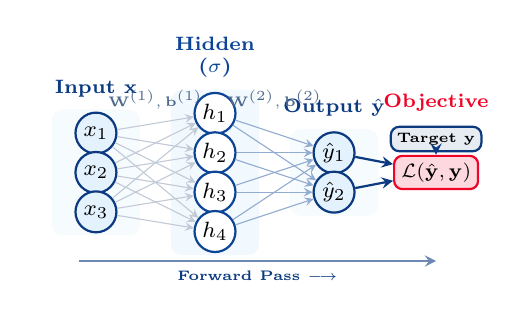
\begin{tikzpicture}[
        x=1.08cm, y=0.50cm, >=stealth,
        neuron_in/.style={circle, draw=cvnavy, fill=cvlightblue!30, thick, inner sep=0pt, minimum size=5.2mm},
        neuron_hid/.style={circle, draw=cvvividblue, fill=white, thick, inner sep=0pt, minimum size=5.2mm},
        neuron_out/.style={circle, draw=cvnavy, fill=cvlightblue!30, thick, inner sep=0pt, minimum size=5.2mm},
        loss_box/.style={rectangle, rounded corners=3pt, draw=cvred, fill=cvred!15, thick, inner sep=2.5pt, font=\scriptsize\bfseries},
        target_box/.style={rectangle, rounded corners=3pt, draw=cvnavy, fill=cvnavy!10, thick, inner sep=2.2pt, font=\tiny\bfseries},
        layer_tag/.style={text width=1.5cm, text centered, font=\scriptsize\bfseries}
      ]
        % Background Layer Backdrops
        \draw[rounded corners=4pt, fill=cvlightblue!10, draw=none] (-0.52, 0.2) rectangle (0.52, 3.4);
        \draw[rounded corners=4pt, fill=cvlightblue!15, draw=none] (0.88, -0.3) rectangle (1.92, 3.9);
        \draw[rounded corners=4pt, fill=cvlightblue!10, draw=none] (2.28, 0.7) rectangle (3.32, 2.9);

        % Input Layer
        \foreach \name / \y in {1/2.8, 2/1.8, 3/0.8}
          \node[neuron_in] (I-\name) at (0, \y) {\footnotesize $x_\name$};

        % Hidden Layer (ReLU)
        \foreach \name / \y in {1/3.3, 2/2.3, 3/1.3, 4/0.3}
          \node[neuron_hid] (H-\name) at (1.4, \y) {\footnotesize $h_\name$};

        % Output Layer
        \foreach \name / \y in {1/2.3, 2/1.3}
          \node[neuron_out] (O-\name) at (2.8, \y) {\footnotesize $\hat{y}_\name$};

        % Target and Loss Node
        \node[target_box] (Target) at (4.0, 2.65) {Target $\mathbf{y}$};
        \node[loss_box] (L) at (4.0, 1.8) {$\mathcal{L}(\hat{\mathbf{y}}, \mathbf{y})$};

        % Connect Input to Hidden
        \foreach \source in {1,2,3}
          \foreach \dest in {1,2,3,4}
            \draw[->, draw=cvmuted!35, thin] (I-\source) -- (H-\dest);

        % Connect Hidden to Output
        \foreach \source in {1,2,3,4}
          \foreach \dest in {1,2}
            \draw[->, draw=cvvividblue!45, thin] (H-\source) -- (O-\dest);

        % Connect Output and Target to Loss
        \draw[->, thick, cvnavy] (O-1) -- (L);
        \draw[->, thick, cvnavy] (O-2) -- (L);
        \draw[->, dashed, thick, cvnavy] (Target) -- (L);

        % Layer Headers
        \node[layer_tag, text=cvnavy, above=0.06cm of I-1] {Input $\mathbf{x}$};
        \node[layer_tag, text=cvvividblue, above=0.06cm of H-1] {Hidden ($\sigma$)};
        \node[layer_tag, text=cvnavy, above=0.06cm of O-1] {Output $\hat{\mathbf{y}}$};
        \node[font=\scriptsize\bfseries, text=cvred, above=0.06cm of Target] {Objective};
        
        % Weights labels
        \node[font=\tiny\bfseries, text=cvmuted] at (0.7, 3.65) {$\mathbf{W}^{(1)}, \mathbf{b}^{(1)}$};
        \node[font=\tiny\bfseries, text=cvmuted] at (2.1, 3.65) {$\mathbf{W}^{(2)}, \mathbf{b}^{(2)}$};

        % Forward flow indicator
        \draw[->, thick, cvnavy!60] (-0.2, -0.45) -- node[below, font=\tiny\bfseries, text=cvnavy] {Forward Pass $\longrightarrow$} (4.0, -0.45);
      \end{tikzpicture}
      \vspace{-0.3em}
      \captionof{figure}{\small Forward computational mapping \& loss evaluation.}
    \end{column}
  \end{columns}
\end{frame}

% ----------------------------------------------------------
% SLIDE 4: Training: Walking the 3D Loss Surface
% ----------------------------------------------------------
\begin{frame}{Training: Walking the Loss Surface}
  \begin{columns}[T,onlytextwidth]
    \begin{column}{0.46\textwidth}
      \begin{block}{Gradient Descent Optimization}
        Minimize scalar error $\mathcal{L}(\hat{\mathbf{y}}, \mathbf{y})$ by stepping along the negative gradient:
        \vspace{-0.2em}
        \begin{equation*}
          \mathbf{w}_{t+1} = \mathbf{w}_t - \eta \nabla_\mathbf{w} \mathcal{L}
        \end{equation*}
        \vspace{-0.2em}
        \begin{itemize}
          \setlength{\itemsep}{0.22em}
          \item High-dimensional surfaces feature complex ravines, valleys, and saddle points.
          \item Hand-derived $\nabla_\mathbf{w} \mathcal{L}$ is intractable for large neural architectures.
          \item \textbf{Core Need}: Fast, memory-efficient automatic gradient computation.
        \end{itemize}
      \end{block}
    \end{column}

    \begin{column}{0.52\textwidth}
      \centering
      \vspace{-0.4em}
      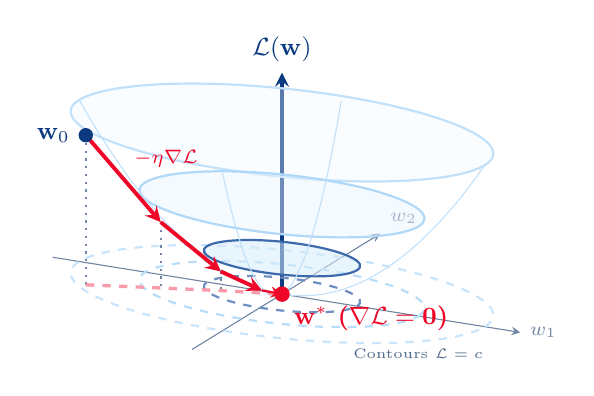
\begin{tikzpicture}[
        x={(1.12cm,-0.18cm)}, y={(0.52cm,0.32cm)}, z={(0cm,0.76cm)},
        >=stealth
      ]
        % Ground Plane Axes (Parameter Space)
        \draw[->, thin, cvmuted!80] (-2.6,0,0) -- (2.7,0,0) node[right, font=\scriptsize\bfseries] {$w_1$};
        \draw[->, thin, cvmuted!80] (0,-2.2,0) -- (0,2.4,0) node[above right, font=\scriptsize\bfseries] {$w_2$};
        \draw[->, very thick, cvnavy] (0,0,0) -- (0,0,3.7) node[above, font=\small\bfseries] {$\mathcal{L}(\mathbf{w})$};

        % 2D Iso-loss Contours on parameter floor (z=0)
        \draw[thick, dashed, cvlightblue!60] (0,0,0) ellipse [x radius=2.3, y radius=1.45];
        \draw[thick, dashed, cvlightblue!80] (0,0,0) ellipse [x radius=1.55, y radius=0.98];
        \draw[thick, dashed, cvvividblue!60] (0,0,0) ellipse [x radius=0.85, y radius=0.54];
        \node[font=\tiny, text=cvmuted] at (2.1, -1.2, 0) {Contours $\mathcal{L} = c$};

        % 3D Loss Surface Shaded Bowls (Tiers)
        \draw[thick, cvlightblue!70, fill=cvlightblue!15, fill opacity=0.35] (0,0,2.7) ellipse [x radius=2.3, y radius=1.45];
        \draw[thick, cvlightblue!90, fill=cvlightblue!25, fill opacity=0.45] (0,0,1.5) ellipse [x radius=1.55, y radius=0.98];
        \draw[thick, cvvividblue!80, fill=cvlightblue!45, fill opacity=0.55] (0,0,0.60) ellipse [x radius=0.85, y radius=0.54];
        
        % Parabolic Profile Curvature Ribs
        \draw[domain=-2.3:2.3, samples=30, smooth, thin, cvlightblue!70] plot (\x, 0, {0.51*\x*\x});
        \draw[domain=-1.45:1.45, samples=30, smooth, thin, cvlightblue!70] plot (0, \x, {1.25*\x*\x});

        % Gradient Descent Path 3D Points
        \coordinate (P0) at (-1.9, -0.70, 2.5);
        \coordinate (P1) at (-1.18, -0.42, 1.10);
        \coordinate (P2) at (-0.60, -0.20, 0.32);
        \coordinate (P3) at (-0.20, -0.06, 0.04);
        \coordinate (Pmin) at (0, 0, 0);

        % Vertical Guideline Drops from 3D to 2D Floor
        \draw[dotted, thick, cvmuted!80] (P0) -- (-1.9, -0.70, 0);
        \draw[dotted, thick, cvmuted!80] (P1) -- (-1.18, -0.42, 0);
        \draw[dotted, thick, cvmuted!80] (P2) -- (-0.60, -0.20, 0);

        % Projected Shadow Path on parameter floor (z=0)
        \draw[dashed, very thick, cvred!40] (-1.9, -0.70, 0) -- (-1.18, -0.42, 0) -- (-0.60, -0.20, 0) -- (0,0,0);

        % Descent Steps in Bold Red
        \draw[->, line width=1.4pt, cvred] (P0) -- node[above right, font=\scriptsize\bfseries, text=cvred] {$-\eta \nabla \mathcal{L}$} (P1);
        \draw[->, line width=1.4pt, cvred] (P1) -- (P2);
        \draw[->, line width=1.4pt, cvred] (P2) -- (P3);
        \draw[->, thick, cvred] (P3) -- (Pmin);

        % Highlighted Points
        \fill[cvnavy] (P0) circle (2.6pt) node[left=0.08cm, font=\small\bfseries] {$\mathbf{w}_0$};
        \fill[cvred] (Pmin) circle (2.8pt) node[below right=0.04cm, font=\small\bfseries, text=cvred] {$\mathbf{w}^*$ ($\nabla \mathcal{L} = \mathbf{0}$)};
      \end{tikzpicture}
      \vspace{-0.3em}
      \captionof{figure}{\footnotesize 3D Convex Loss Bowl \& Gradient Trajectory.}
    \end{column}
  \end{columns}
\end{frame}

% ----------------------------------------------------------
% SLIDE 5: The ML Dilemma: Heavy Frameworks vs. Small Models
% ----------------------------------------------------------
\begin{frame}{The ML Dilemma: Heavy Frameworks vs. Small Models}
  \begin{columns}[T,onlytextwidth]
    \begin{column}{0.48\textwidth}
      \begin{block}{The Industry Reality}
        \begin{itemize}
          \setlength{\itemsep}{0.35em}
          \item Mainstream deep learning frameworks are built for datacenter-scale LLMs and massive clusters.
          \item \textbf{The Mismatch}: Most industrial, edge, and educational workloads rely on \textbf{compact models} (MLPs, small CNNs, PINNs).
          \item Multi-gigabytes required just to train or evaluate a lightweight neural network.
          \item High barrier of entry for students, independent researchers, and low-compute laboratories.
        \end{itemize}
      \end{block}
    \end{column}

    \begin{column}{0.48\textwidth}
      \begin{alertblock}{The Practical Barriers}
        \begin{itemize}
          \setlength{\itemsep}{0.35em}
          \item \textbf{Cloud \& Serverless}: Crippling cold starts downloading gigabytes of container images on ephemeral workers.
          \item \textbf{Edge \& IoT Deployment}: Incapable of running on constrained micro-controllers or low-power embedded hardware.
          \item \textbf{Resource Overhead}: Excessive RAM and energy footprint for straightforward computational tasks.
          \item \textbf{Dependency Fragility}: Heavy, opaque C++ runtimes that complicate cross-platform setups.
        \end{itemize}
      \end{alertblock}
    \end{column}
  \end{columns}
\end{frame}

% ----------------------------------------------------------
% SLIDE 6: The Pedagogical Crisis: Peeling the Black Box
% ----------------------------------------------------------
\begin{frame}{The Pedagogical Crisis: Peeling the Black Box}
  \begin{columns}[T,onlytextwidth]
    \begin{column}{0.50\textwidth}
      \begin{alertblock}{The Black Box Problem in AI Education}
        \begin{itemize}
          \setlength{\itemsep}{0.25em}
          \item Mainstream frameworks encapsulate execution within opaque, pre-compiled C++ binaries.
          \item Learners frequently invoke high-level APIs without exposure to Jacobians, gradient routing, or computation graphs.
          \item Standard documentation prioritizes \textbf{API signatures} over foundational mathematical derivations.
        \end{itemize}
      \end{alertblock}
    \end{column}

    \begin{column}{0.46\textwidth}
      \begin{exampleblock}{The Call for Democratization}
        \begin{itemize}
          \setlength{\itemsep}{0.25em}
          \item \textbf{Mathematical Transparency}: Complete comprehension requires understanding tensor transformations from first principles.
          \item \textbf{Universal Accessibility}: Empowering researchers and students globally to innovate without requiring high-end GPU clusters.
        \end{itemize}
      \end{exampleblock}
      \vspace{0.4em}
      \begin{center}
        \textbf{Enter Sorix}: Combining minimal compute with complete mathematical openness.
      \end{center}
    \end{column}
  \end{columns}
\end{frame}

% ----------------------------------------------------------
% SLIDE 7: The Genesis of Sorix
% ----------------------------------------------------------
\begin{frame}{The Genesis of Sorix: Minimalist \& Accessible}
  \begin{columns}[T,onlytextwidth]
    \begin{column}{0.49\textwidth}
      \begin{block}{The Sorix Philosophy}
        Conceived to train and deploy neural networks with \textbf{maximum efficiency} on commodity hardware without binary bloat.
        \vspace{0.25em}
        
        \textbf{Core Architectural Pillars}:
        \begin{itemize}
          \setlength{\itemsep}{0.08em}
          \item \textbf{PyTorch Parity}: Zero learning curve for researchers.
          \item \textbf{Dual Backend}: Native NumPy (CPU) + CuPy (GPU).
          \item \textbf{Zero C++ Build}: Instant cross-platform deploy.
          \item \textbf{Production Ready}: Native model serialization.
        \end{itemize}
      \end{block}
    \end{column}

    \begin{column}{0.47\textwidth}
      \begin{exampleblock}{Isolated Environment Size}
        \centering
        \scriptsize
        \begin{tabular}{lrr}
          \toprule
          \textbf{Framework} & \textbf{CPU Size} & \textbf{GPU Size} \\
          \midrule
          \rowcolor{cvlightblue!35}
          \textbf{Sorix} & \textbf{54 MB} & \textbf{238 MB} \\
          PyTorch & 702 MB & 6{,}840 MB \\
          TensorFlow & 1{,}406 MB & 1{,}978 MB \\
          \bottomrule
        \end{tabular}
      \end{exampleblock}
      \vspace{-0.4em}
      \begin{alertblock}{Massive Footprint Advantage}
        \footnotesize \textbf{$13\times$--$26\times$ footprint reduction} on CPU and \textbf{$28\times$} on GPU vs.\ heavy runtimes.
      \end{alertblock}
    \end{column}
  \end{columns}
\end{frame}

% ----------------------------------------------------------
% ----------------------------------------------------------
% SLIDE 8: The Sorix Ecosystem: Ready for Global Use
% ----------------------------------------------------------
\begin{frame}{The Sorix Ecosystem: Ready for Global Use}
  \begin{columns}[T,onlytextwidth]
    \begin{column}{0.48\textwidth}
      \begin{block}{Distribution \& Installation}
        \begin{itemize}
          \setlength{\itemsep}{0.32em}
          \item \textbf{PyPI Standard Package}:\\
            \texttt{pip install sorix}
          \item \textbf{CUDA GPU Acceleration}:\\
            \texttt{pip install "sorix[cp13]"}
          \item \textbf{Open-Source Codebase}:\\
            \href{https://github.com/Mitchell-Mirano/sorix}{\texttt{Mitchell-Mirano/sorix}}
          \item \textbf{License}: Permissive Open Source (MIT)
        \end{itemize}
      \end{block}
    \end{column}

    \begin{column}{0.48\textwidth}
      \begin{exampleblock}{Rigorous Documentation \& Tutorials}
        \begin{itemize}
          \setlength{\itemsep}{0.32em}
          \item \textbf{Mathematical Derivations}: Every layer, loss, and backward pass is fully derived with LaTeX proofs.
          \item \textbf{Physics \& PINNs}: Interactive Google Colab tutorials for differential equations and deep learning.
          \item \textbf{Official Platform}: Fully accessible at \href{https://sorix.mitchellmirano.com}{\texttt{sorix.mitchellmirano.com}} (scannable via final QR code).
        \end{itemize}
      \end{exampleblock}
    \end{column}
  \end{columns}
\end{frame}

% ----------------------------------------------------------
% SLIDE 9: Dual Hardware Engine & Benchmarks
% ----------------------------------------------------------
\begin{frame}[fragile]{Dual Hardware Engine \& Empirical Benchmarks}
  \begin{columns}[T,onlytextwidth]
    \begin{column}{0.44\textwidth}
      \begin{block}{NumPy on CPU, CuPy on GPU}
        \begin{itemize}
          \item Dynamic routing with zero C++ compilation.
          \item Transparent GPU acceleration:
        \end{itemize}
        \lstset{style=pythonstyle, basicstyle=\ttfamily\fontsize{5.8pt}{6.8pt}\selectfont}
        \begin{lstlisting}
# GPU acceleration (CuPy CUDA)
x = tensor([1.0, 2.0]).to("cuda")

# CPU edge execution (NumPy)
x = tensor([1.0, 2.0]).to("cpu")
        \end{lstlisting}
      \end{block}
    \end{column}

    \begin{column}{0.54\textwidth}
      \textbf{MNIST Benchmark (5 Epochs)}:
      \vspace{0.2em}
      \begin{table}[ht]
        \centering
        \scriptsize
        \setlength{\tabcolsep}{3.5pt}
        \begin{tabular}{llrrr}
          \toprule
          \textbf{Framework} & \textbf{Device} & \textbf{Train Time} & \textbf{Inference} & \textbf{Acc} \\
          \midrule
          \rowcolor{cvlightblue!35}
          \textbf{Sorix} & \textbf{CPU} & \textbf{7.36s} & \textbf{0.032s} & \textbf{97.2\%} \\
          PyTorch & CPU & 9.21s & 0.048s & 97.4\% \\
          TensorFlow & CPU & 17.14s & 0.186s & 96.8\% \\
          \addlinespace
          \rowcolor{cvred!15}
          \textbf{Sorix} & \textbf{GPU} & \textbf{6.21s} & \textbf{0.015s} & \textbf{97.6\%} \\
          PyTorch & GPU & 4.04s & 0.025s & 97.6\% \\
          \bottomrule
        \end{tabular}
      \end{table}
      \footnotesize \textbf{Sorix CPU training is 20\% faster} than PyTorch with the lowest batch latency.
    \end{column}
  \end{columns}
\end{frame}

% ----------------------------------------------------------
% SLIDE 10: PyTorch Compatibility: Zero Learning Curve
% ----------------------------------------------------------
\begin{frame}[fragile]{PyTorch Compatibility: Zero Learning Curve}
  \begin{columns}[T,onlytextwidth]
    \begin{column}{0.53\textwidth}
      \begin{block}{Canonical Deep Learning Pipeline in Sorix}
        \lstset{style=pythonstyle, basicstyle=\ttfamily\fontsize{6.2pt}{7.2pt}\selectfont}
        \begin{lstlisting}
from sorix.nn import Sequential, Linear, ReLU, MSELoss
from sorix.optim import SGD

# 1. Modular Model Definition
model = Sequential(
    Linear(784, 128),
    ReLU(),
    Linear(128, 10)
)
criterion = MSELoss()
optimizer = SGD(model.parameters(), lr=0.01)

# 2. Canonical Training Iteration
for epoch in range(epochs):
    optimizer.zero_grad()
    loss = criterion(model(X), y)
    loss.backward()   # Backward loss propagation
    optimizer.step()  # In-place parameter update
        \end{lstlisting}
      \end{block}
    \end{column}

    \begin{column}{0.44\textwidth}
      \begin{exampleblock}{Zero Learning Curve}
        \begin{itemize}
          \setlength{\itemsep}{0.1em}
          \item \textbf{1:1 Mental Model}: If you know PyTorch, you already know Sorix.
          \item \textbf{Identical API}: Same classes, training loop, and optimizers.
        \end{itemize}
      \end{exampleblock}

      \begin{alertblock}{54 MB Micro-Engine Advantage}
        \begin{itemize}
          \setlength{\itemsep}{0.1em}
          \item \textbf{$126\times$ Lighter}: Full workflow without multi-GB binaries.
          \item \textbf{Pure Transparency}: Tensors and gradients are accessible NumPy/CuPy arrays with zero black boxes.
        \end{itemize}
      \end{alertblock}
    \end{column}
  \end{columns}
\end{frame}

% ----------------------------------------------------------
% SLIDE 11: Conclusion & Contact
% ----------------------------------------------------------
\begin{frame}[plain]
  \centering
  \vfill
  {\bfseries\fontsize{24pt}{28pt}\selectfont Thank You for Your Attention!}\\[0.45em]
  {
\includegraphics[height=1.35em]{images/spasibo.pdf}}\\[1.0em]

  \begin{columns}[T,onlytextwidth]
    \begin{column}{0.46\textwidth}
      \centering
      \begin{block}{\centering Mitchell Mirano Caro}
        \centering\vspace{0.4em}
        \colorbox{white}{\setlength{\fboxsep}{4pt}\textcolor{black}{\qrcode[height=2.2cm,nolink]{https://mitchellmirano.com}}}\\[0.4em]
        \textbf{Personal Portfolio \& CV}\\[0.1em]
        \href{https://mitchellmirano.com}{\textbf{\small mitchellmirano.com}}
      \end{block}
    \end{column}
    \begin{column}{0.46\textwidth}
      \centering
      \begin{exampleblock}{\centering Sorix Deep Learning Engine}
        \centering\vspace{0.4em}
        \colorbox{white}{\setlength{\fboxsep}{4pt}\textcolor{black}{\qrcode[height=2.2cm,nolink]{https://sorix.mitchellmirano.com}}}\\[0.4em]
        \textbf{Documentation \& Benchmarks}\\[0.1em]
        \href{https://sorix.mitchellmirano.com}{\textbf{\small sorix.mitchellmirano.com}}
      \end{exampleblock}
    \end{column}
  \end{columns}

  \vspace{0.9em}
  {\fontsize{12pt}{15pt}\selectfont \textbf{Questions and Comments are Welcome!}}
  \vfill
\end{frame}

\end{document}
